\documentclass{article}
\usepackage{graphicx}^^M
\graphicspath{{images/}}
\usepackage{fancyhdr}
\usepackage[svgnames]{xcolor}
\definecolor{StevensRed}{RGB}{163,38,56}
\definecolor{StevensGray}{RGB}{154,152,154}

\usepackage[english]{babel}
\usepackage[utf8]{inputenc}
\usepackage{indentfirst}
\usepackage{caption}
\usepackage{subcaption}

\usepackage{hyperref}
\hypersetup{
    colorlinks=true,
    linkcolor=StevensRed,
    filecolor=StevensGray,      
    urlcolor=StevensRed
}



\usepackage[paper=a4paper,top=0in,bottom=0in,right=0in,left=0in]{geometry}
\begin{document}

\title{Stevens Athletics Documentation}
\begin{titlepage}

    
\includegraphics[width = 250px]{images/stevensLogoChevron.png}
    \vspace{1.5cm}
    \begin{center}
	{\scshape\LARGE Stevens Athletics Event Staff Documentation\par}
	\vspace{0.5cm}
	{\scshape A Complete Guide to Running the Games \par}
    \vspace{1cm}
    \vfill
    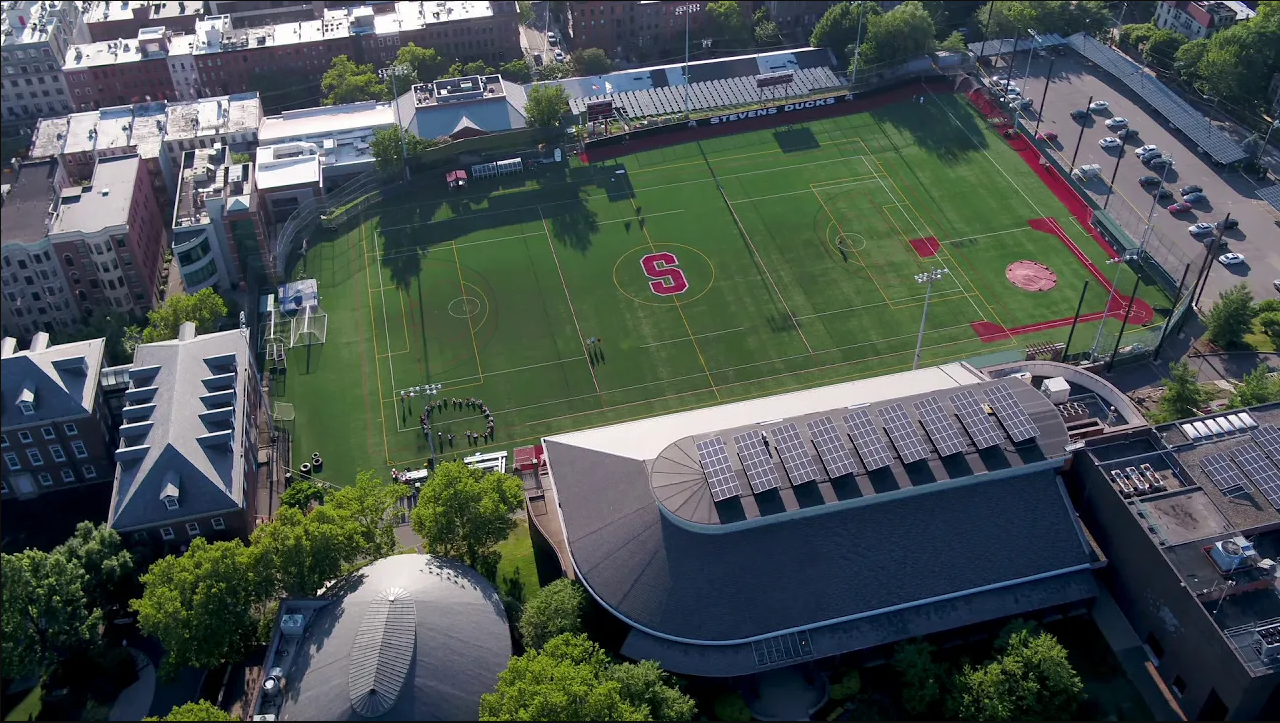
\includegraphics[viewport=125 50 750 600]{images/field.png}]
    \end{center}
\end{titlepage}

\newgeometry{margin=1in}
\pagestyle{fancy}
\fancyhf{}
\rhead{Athletics Event Staff}
\rfoot{Page \thepage}
\pagenumbering{roman}
\lhead{Introduction and Positions}
\renewcommand{\headrulewidth}{1pt}
\renewcommand{\footrulewidth}{1pt}

\section{Introduction}
The overall mission of the Stevens Institute of Technology Department of Physical Education, Athletics and Recreation is to enhance the healthy lifestyles of all members of the Stevens community through providing programs, facilities and training that promote physical fitness, competition and life-skill development. The Athletics Event Staff aid the Athletics Department in setting up, breaking down, and game day duties for each of the hosted games played at Stevens Institute of Technology. As a member of the staff, each worker helps ensure the quality, fairness, and accessibility of sporting events hosted at Stevens Institute of Technology is at the highest standard. Our flexible scheduling is ideal for students looking for ways to receive their Financial Work Study hours, however, please note that workers are expected to sign up for open positions each week and be willing to commit regular hours to the job. 

\paragraph{As a member you are expected to:}
\begin{itemize}
    \item Have the ability to work independently.
    \item Be willing to stand for extended periods of time without sitting.
    \item Give and take direction from different workers, supervisors and managers in a professional manner.
    \item Work outside in varying weather conditions.
    \item Sign up for events in advance and show up in a timely fashion
\end{itemize}

\tableofcontents
\newpage

\section{Job Positions}
At Stevens Institute of Technology, the following sports are hosted during the following seasons: 

\def\arraystretch{1.25}
\begin{table}[h]
    \centering
    \begin{tabular}{c|c|c}
        Fall & Winter & Spring\\
        \hline
        Soccer & Swimming & Baseball\\
         & Basketball & Lacrosse\\
         & Wrestling & Volleyball\\
        & & \\
    \end{tabular}
    \caption{Men's Sports}
\end{table}

\begin{table}[h]
    \centering
    \begin{tabular}{c|c|c}
        Fall & Winter & Spring\\
        \hline
        Soccer & Swimming & Softball\\
        Volleyball & Basketball & Lacrosse\\
        Field Hockey & & \\
        & & \\
    \end{tabular}
    \caption{Women's Sports}
\end{table}

    As a member of the Athletics Event Staff it is your duty to fill the positions needed for each hosted game at Stevens Institute of Technology. These jobs are:
    
\def\arraystretch{2}
\begin{table}[h]
    \centering
    \begin{tabular}{cccc}
        Event Setup & Ball Runner & Gate Collection & Music Operator \\
        Statistics Spotter & Statistics Typist & Webcast Producer & Camera Operator\\
        
    \end{tabular}
\end{table}

The remainder of this document will explain the expectations for each job and act as an in-depth resource manual to explain  each job in full detail.
\newpage
\pagenumbering{arabic}

%---------- Start writing here -----------------%
\lhead{Job Descriptions}

%---------- Setup and Breakdown -----------------%
\section{Event Setup and Breakdown}

%---------- Gate Collection -----------------%
\section{Gate Collection}
Gate collection fees are crucial for funding the athletic events at Stevens Institute of Technology. The money made from entrance fees are able to give better opportunities to the athletes competing. When in charge of gate collection, it is the worker’s responsibility to check all spectators coming to the games to make sure they do not enter without first paying. Gate collection is also the first contact Stevens Athletics Events Staff has with spectators and we look to welcome spectators to the sports in a respectable manner.
\newline

Staff in charge of gate collection should report earlier than most positions in order to man the entrances for spectators. Gate collectors are therefore expected to arrive one hour and thirty minutes before the event takes place and are stationed at their position until halftime of most games. Depending on the amount of staff, one or two may be placed at each station and the amount of stations may vary. Usually, there are four gate collectors, two at each entrance for both indoor and outdoor events.
\newline

 \subsection{Schaefer Center Canavan Arena}
At indoor events, gate collectors are placed outside of the entrances to the Shaefer Center Canavan Arena. Tables should already be prepared by their arrival by the setup staff, but if not, the tables and chairs are both stored near the exit to the outdoor stands. See the appendix for more information.

% ADD APPENDIX LINK FOR TABLES AND CHAIRS HERE %

At indoor events, gate collectors are also put in charge of distributing the programs for the event. They should be given a pile for people interested to take. Usually, these can be left at the edge of the table in view of the spectators entering and they will grab one if interested. 

%(image of setup for gate collection)%

Pricing and Distribution:
When gate collectors arrive, they should report to Keith in order to pick up their materials and head to their respective tables. They should receive a laminated pricing guide to place at the entrances, a small safe to keep money secure and a roll of tickets. See the appendix for more information. 

% ADD APPENDIX LINK FOR SAFES AND LAMINATED PAPERS %

At Stevens, students, faculty, and parents of Stevens athletes are exempt from paying for entrance into the games. For Stevens students, staff should check for ID confirmation if unsure. For parents of Stevens athletes, gate collectors will usually be provided with a list of people allowed to enter free of charge. If this list is not provided, the workers can ask for the student’s (athlete) name and check the Stevens roster on the programs for confirmation. Otherwise, all other admission prices are laid out on the laminated paper seen below. General admission is \$5, while senior citizens and non-Stevens students are \$3. Before entering, each paying member should be given a ticket from the roll provided in order. The tickets have two parts, one to give out and one to keep in order to track how many tickets were sold. 

\subsection{Dobbelarr Field}
At outdoor events, gate collectors are stationed near the entrance to the field near Kidde 228 (2) as well as near the entrance to the bleachers on the opposite side near the parking lot (1) . If there are enough workers, a third table is sometimes used near the exit from the Schaefer Gym (3). See the map below. At halftime, the gate collection staff should locate Keith in order to hand back the supplies and money made. 

\begin{figure}[h]
\begin{center}
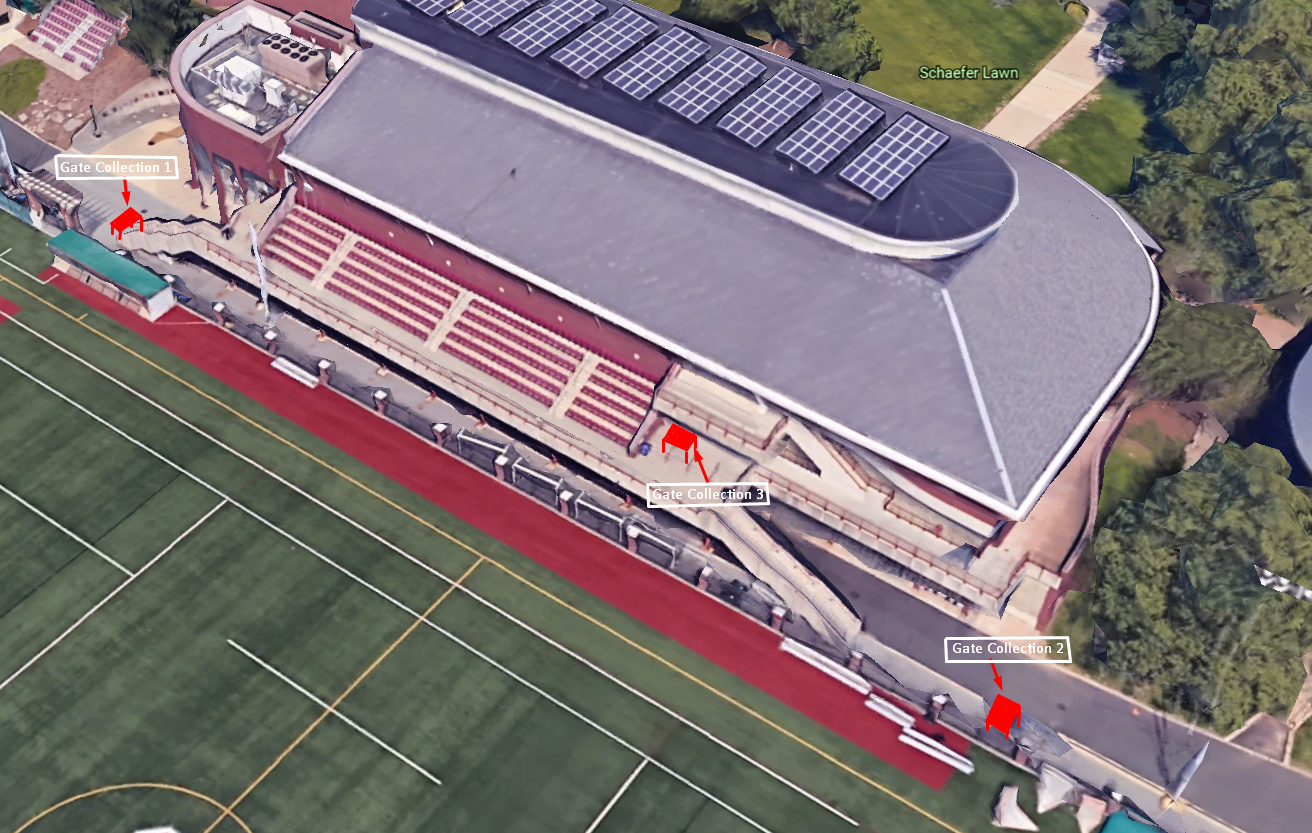
\includegraphics[width=400px]{images/GateCollections.png}
\caption{The three locations for Dobbelarr Field Gate Collection}
\end{center}
\end{figure}

Miscellaneous:
Sometimes, gate collection is given the opportunity to hand out Stevens clothing for season openers or specific events. In these cases, the tables should be given prior notice and be told how they should be distributed. 
\newline

Furthermore, during championship games, Stevens students and parents of athletes are unfortunately not given the ability to enter for free. However, the Athletics staff looks to take over the cost of Stevens students tickets by paying themselves in order to fill the games with more supporting fans. During championship games, gate collection should also keep track of the Stevens students entering separately and should hand out tickets to them in order to do so. A separate pile of the “Keep this Side” raffle tickets should be kept to account for all the Stevens students that came to watch the game.  

%---------- Webcast Producer -----------------%
\section{Webcast Producer}
All games run by the Stevens Athletics staff are live streamed to the public watching at home. In order to do this, a webcast producer is needed at each game in order to update the scores and times for the game in real-time. The webcast producer is expected to show up an hour before the scheduled game time to make sure everything is set up accordingly and that they are prepared before the game begins. If this is your first time doing webcast, come more than an hour early in order to properly ask questions and learn to run the broadcast effectively. 

\subsection{Setup Webcast}
It is the webcast producer’s responsibility to have a computer setup in order to correctly stream the games live through the internet. They should work with the camera operator in order to bring out supplies and correctly connect all the cables to the camera and laptops. All of the webcast supplies are stored within the office on the second floor. See the appendix for more information on each of the setup cables and electronics. 

%{Link to duffel bag for webcast}%

When working in Canavan, there should be a white table setup on the bleachers for you to set up on. When working outside in the announcer box, the webcast works against the right wall, near the camera operator on their own separate table. Please use the appendix links to see what the objects referenced look like. This section will go more in depth on where the connections should be made. 

%{Image of full complete setup both inside and outside}%

As you can see from the image, there are multiple wires and electronics that the webcast producer is in charge of. Not only does the laptop need to accurately stream the image from the camera, but the webcast must also stream the audio from the play-by-play announcer sitting nearby. 

\subsubsection{Laptop Setup}
Take the laptop found within the bag and place it on the left side of the table. The basic setup at the table should be, laptop on the left, camera in the middle, and mixer on the right. There are multiple cables that need to be connected to power, so one of the first things that should be taken out is the extension cord/power strip. The laptop needs its charger to make sure it does not run out of battery throughout the game and should be connected into the power strip. Similarly, the laptop needs to be connected to the internet through Ethernet instead of a wireless connection. Ethernet allows the computer to run a faster and more stable connection and has a smaller chance of failing during the game.

%{Image of laptop connections}%

Next, the camera needs to be connected to the laptop. The camera operator should have an HDMI cable running out of the camera. This HDMI cable needs to be converted into an input for the computer, so it needs to run through a capture device. When plugged in correctly, you should see a white light on the capture device. See appendix for more details.

%{Image of capture device and correct connections}%

Finally, the mixer needs to be connected to the laptop to stream audio in the webcast. The physical mixer should be within the bag and should be placed at the right side of the table. Along with it, a headset should be taken out an prepared for the play-by-play announcer. This headset should be connected into the Microphone 1 slot of the mixer. The mixer also needs to be connected to power and to the laptop. The charger should be connected to the power strip and a USB cable connects the mixer to the laptop. 

%{Image of the mixer correctly set up}%

\subsection{Working with Wirecast}
The Stevens Athletics staff uses Wirecast to stream to the spectators that are not at the game. Wirecast is available on the laptop and multiple templates are pre-made for different game types. Double click on the Wirecast logo to open up the program and using the file tab, open the most recent file. This will open up the previous template and changes will have to be made for the new game.

%Wirecast logo%

On the left side of the screen there should be a circle with three dots in it. This allows you to see all the information that is displayed on the overlays on the screen. Anything from the time and score, to the team names and colors can be changed. You will need to update the information before the game starts depending on which teams are playing. 
\newline 

The team name should be updated based on the game and the team color should be changed. Usually, team colors can be found by searching the university’s color scheme. There is also a line that has information about the game and it should be updated to the correct timing (quarters or halves) for the sport being played and also the name of the location. This is either Canavan Arena or Dobbelaar Field. Once the camera is set up, the camera operator should communicate with the webcast producer to make sure the stream is in focus and centered. Similarly, once the play-by-play announcer arrives, make sure the sound is passing through and not being distorted. There is an audio indicator on Wirecast that can be checked to make sure the audio is working. 

%{image of correct overlays and editing screen}%

\subsection{Live Updates}
The webcast usually starts 5-15 minutes before the actual game begins. In order to turn on the webcast, hit the symbol that looks like a WiFi signal on the top of the stream. It should turn green to indicate it is on. 

%{image of the WiFi symbol}%

Once a game begins, it is the webcast producer’s duty to follow through the game and update the score and time. The time overlay should be updated every minute, while the score should be updated to reflect the live score displayed on the scoreboard. 
\newline

At halftime, the play-by-play announcer will momentarily sign off to allow for videos to be played. After the announcer finishes, the mixer should be muted and videos should be played for halftime. The halftime videos are found at the bottom of the screen. The NCAA, Empire 8 and Stevens Athletics videos should be played one after another (if there is less time in the half then you do not have to play the Stevens video). You need to manually click from one video to the next, so you should pay attention to when you will need to be changing them. After the videos are done, you should also play highlights that have been captured throughout the first half. 
\newline

As a general rule of thumb, you should plan to have the halftime videos end with about 2 minutes left in the half so that you can start getting set up for the next half and for the play-by-play announcer to be introduced back in.
\newline

Once the game ends, wait for the play-by-play announcer to finish his recap of the game and sign off. Then, click the stream button (WiFi symbol) to end the stream and go to file and hit save (no need for save as). Close the Wirecast and begin to pack everything back. 


%---------- Camera Operator -----------------%
\section{Camera Operator}
All games run by the Stevens Athletics staff are live streamed to the public watching at home. In order to do this, a camera operator is needed at each game in order to follow the game’s action and zoom into the most important areas of the field or court. The camera operator is expected to show up an hour before the scheduled game time to make sure everything is set up accordingly and that they are connected to the webcast that is being run. 
\newline 

It is the camera operator’s responsibility to have the camera set up correctly on the tripod and have it connected to the webcast before the game begins. While the setup crew may set up the camera, the camera operator should still know how to setup the camera themselves. The camera, tripod, and necessary cables are all stored within the office. See the appendix for more information. 

% ADD APPENDIX LINK FOR CAMERA, TRIPOD, AND NECESSARY CABLES %

\subsection{Camera Setup}
For a game in Canavan, the camera should be set up on top of the table at the top of the bleachers behind the statistics table. The tripods legs can be opened up but do not have to be lengthened for games within Canavan, as it is standing on a table already. If setting up outside, the camera should be placed in the far right corner of the announcer box and the tripod should be fully extended to the maximum height. Once the tripod is securely fastened and stable, the camera should be placed on the top. The camera slides into the top with buttons on the sides to allow for it to slide through. There should be a red button on the left side which allows it to continue sliding. Once it is at the center of the tripod, tighten the camera into place by twisting the black lever and make sure the camera is locked in. Do not let go of the camera until you have made sure it is securely fastened. 

%{image of putting camera on tripod}%

After the camera is safely placed on the tripod, multiple cables need to be run to and from it in order to have it operate. Each of these cables can be found in the office. See the appendix for more information.

% ADD APPENDIX LINK FOR CAMERA CABLES %

The power cord needs to be plugged in to the bottom right side of the camera. This will give power to the camera and allow it to turn on. This should also be the first step to check if the camera does not turn on. 

%{image of power cable input}%

The tripod also comes with a handle attachment which allows for easier movement of the camera to follow the action in the game. Furthermore, the handle has a dedicated button for zooming into and away from the action when necessary. The remote for the handle is plugged into the left of the power cord. 

%{image of remote handle input}%

The camera also needs to be plugged into the HDMI cable which connects the camera’s feed to the computer that the webcast producer is using. The HDMI signal needs to be converted into a signal that allows the computer to recognize the input, and so it is connected into a capture device that feeds further into the computer’s USB input. 

%{image of HDMI input}%

Once the cables are all situated, the camera operator should look at the image shown on the webcast and change the focus and zoom to make it correctly display to the audience at home. The camera operator is then completely set up and needs to only follow the action as it plays out during the game. 




%---------- Music Operator -----------------%
\section{Music Operator}
A music operator performs all the music and sound prompts that occur during the games. Furthermore, it is the music operators job to play the national anthem before the start of each game and play the correct entrance music for Stevens roster introductions. Music operators should arrive 75 minutes before a game starts in order to play the correct warm up music for sports teams. Furthermore, music cannot and should not be played while the game is underway. The following sections will allow you to learn the ins and outs of the software, hardware, and differences in job requirements between sports.

\subsection{Sound Director}
At Stevens Institute of Technology, Sound Director is used as an instant access soundboard-esque audio solution for sporting events. Sound Director is a very easy to learn program for music operators with limited but valuable commands available for real-time audio adjustment. The main screen is split into three main sections as seen in Figure 1. 

\begin{figure}[h]
\begin{center}
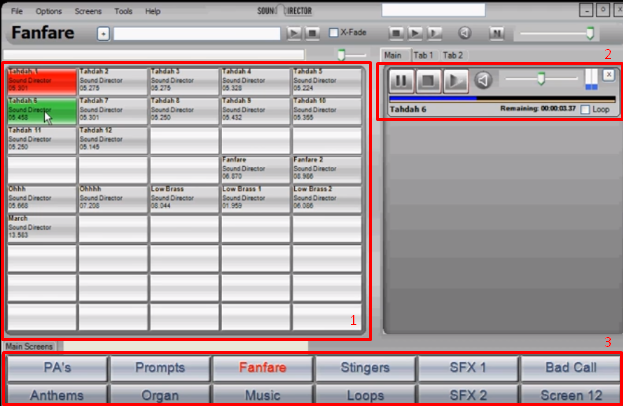
\includegraphics[width=400px]{images/SoundDirector.png}
\caption{\\ 1. Music Selection Screen \\ 2. Music Adjustment Screen \\ 3. Main Screen Selection}
\end{center}
\end{figure}
 
\subsubsection{Music Selection Screen}
In the music selection screen, the music operator can see the multiple buttons for music that can be selected to be played. Each button has the name of the song as well as the length of the song. In order to play music, the music operator only needs to click once and the song will begin to play. As the song is playing, the button will appear green and the music adjustment screen will update to give the user more flexibility with the audio. When the song ends, the button will appear red. Red songs/sound effects are still available to be played, but they help show which songs have already been played to keep operators from playing the same songs multiple times during one event. Finally, if certain music wants to be queued up it can be dragged from the music selection screen to the music adjustment screen.

\subsubsection{Music Adjustment Screen}
The music adjustment screen is filled with blocks of music, each with a collection of adjustments that can be made. Figure 2 is a block within the music adjustment screen created for a selected song.

\begin{figure}[h]
\begin{center}
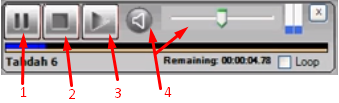
\includegraphics[]{images/adjustment.png}
\caption{The Music Adjustment Screen}
\end{center}
\end{figure}

There are multiple buttons, a slider, and some valuable information on this screen. 

\begin{enumerate}
    \item  Moving from left to right, the first button is the pause/play button. This button allows you to play music that was queued up and also pause music if the music wants to be returned to later. 
    \item The next button is the stop button. The stop button acts similarly to the pause button, except it removes the song from the music adjustment screen entirely. 
    \item The third button is the fade button and is the most important button on this screen. It is highly unlikely that after a timeout or halftime the music ends perfectly with the resuming of play. Because of this, the music is almost always faded out with this button. After fading out, the music is removed from the music adjustment screen. 
    \item The mute button is rarely used, but the volume slider allows for quick adjustments if the music playing is too loud. There are other ways to lower the volume of the music, as well. 
\end{enumerate}

\subsubsection{Main Screen Selection}
The main selection screen is a useful way to organize different types of music into separate screens. At Stevens Athletics, the main screen selection is organized based off of either sport, or based on genre of music. By clicking on each of the screens, more options for music can be found. 

\subsubsection{Hot Keys}
Sometimes it is important to have sound effects bound to specific keys to make them available no matter what main screen is open. This is used most effectively for goal horns, which occur right after a goal is scored in some sports, or a home run in softball and baseball. Because goals cannot be predetermined, music operators should stay focused on the game and react properly to these occurrences. 
\newline
The following sports use goal horns during play:
\begin{itemize}
    \item Soccer
    \item Field Hockey
    \item Lacrosse
    \item Baseball/Softball
\end{itemize}

\subsubsection{iPad Volume Sliders}
When working with the audio system at Dobbelaar Field, the music operator will also have the added volume adjustments through an application called MotionControl on the iPad. After connecting to the appropriate network, the iPad will have access to changing the volume from the wall jack at any outside sporting event. This includes the music as the left most slider, and the microphone as the central slider.

\begin{figure}[h]
\begin{center}
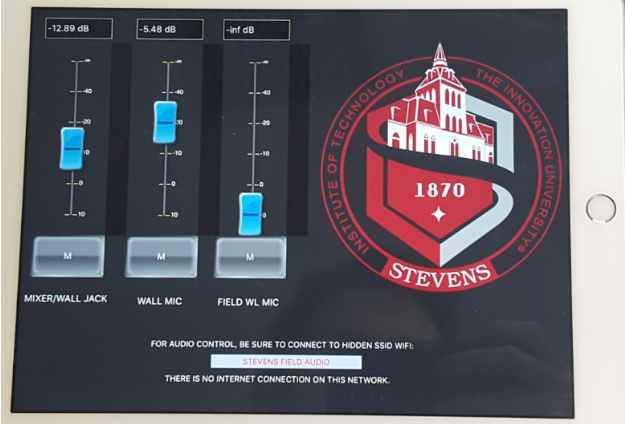
\includegraphics[width= 300px]{images/iPadVolume.png}
\caption{iPad Volume Slider}
\end{center}
\end{figure}

\subsection{Hardware}
As a music operator, there are a few pieces of hardware that would be beneficial to be familiar with as well as knowledge on connections to the general audio system around the field and gymnasium. When working games outside, only a laptop with Sound Director will be used without any further audio equipment. However, the audio output, as well as the microphone need to be connected to the Dobbelaar field audio system to output through the loudspeakers. 

\begin{figure}[h]
\begin{center}
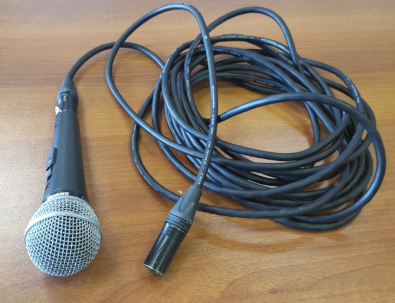
\includegraphics[width=250px]{images/Microphone.png}
\caption{Microphone connects to the audio system output shown below}
\end{center}
\end{figure}

\begin{figure}[h]
\begin{center}
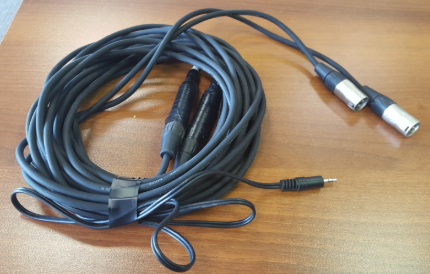
\includegraphics[width=200px]{images/AudioCable.png}
\caption{Audio cable connects to the audio system left and right mixes as well as the headphone jack of the laptop running Sound Director}
\end{center}
\end{figure}

\begin{figure}[h]
\begin{center}
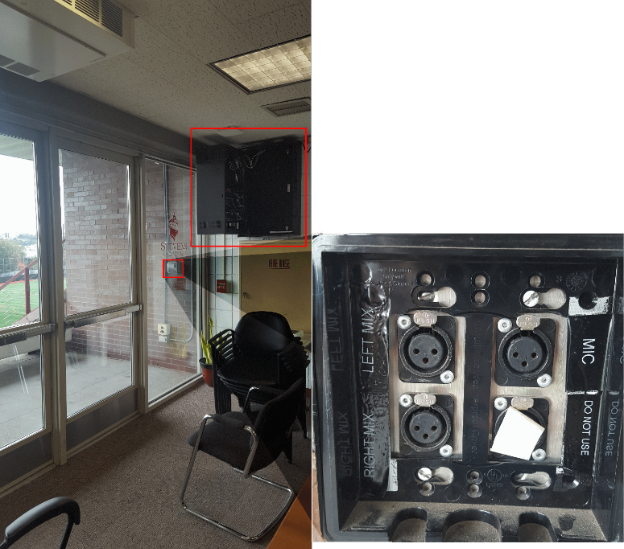
\includegraphics[width=250px]{images/Untitled.png}
\caption{Noted in red are the field audio system outlets and the storage location for the iPad, microphone, and audio output cable.}
\end{center}
\end{figure}

\subsubsection{Differences in Sports}
Members of each sporting team spend a lot of time practicing and warming up before their matches. Some sports teams create music precisely timed in order to go through a flow of different warm up exercises, changing the exercises as the music does. It is imperative to arrive early to be able to set up this music for our athletes.
\newline

Furthermore, each game starts with opening rosters of the teams playing, the national anthem, and a short inspection of rosters and equipment by referees before the games start. These may occur in different orders so one should be prepared to adapt the order of some music like lineups and the national anthem and ask when arriving what the order will be. Each sport should have the proper music under their own music selection screen. 

\section{Statistics Spotting and Typing}
In order to be able to spot statistics or type statistics into the system, members of the Athletic staff need to be trained on the specific software and have a strong understanding of the sport's rules. Due to this, these two positions should not be staffed by students before talking to Charles and being taught how to use the program efficiently and without error. 

\section{Ball Running}

\section{Appendix}
The appendix has valuable information on where items are stored. The appendix can be linked within the document to show where things can be found. Each item has its own description of when it would be used and its location, along with a picture of where it is and how it looks.


\end{document}

%-----ADDING FIGURES------
%\begin{figure}[h]
%\begin{center}
%\includegraphics[width=\textwidth]{IMAGE_NAME_HERE}
%\caption{CAPTION_HERE}
%\end{center}
%\end{figure}

%-----ADDING TABLES-------
%\begin{table}[h]
%\begin{center}
%\begin{tabular}{c|c|c|c|c}
%& Butterworth & Chebyshev & Linkwitz-Riley & Bessel\\
%\hline
%Passband Accuracy & 10 & 4 & 6 & 9\\
%\hline
%Filter Slope & 7 & 10 & 5 & 6\\
%\hline
%Impulse Response & 5 & 7 & 10 & 3\\
%\hline
%Popularity in Crossover Filters & 3 & 3 & 7 & 3\\
%\hline
%Total & 25 & 24 & 28 & 21\\
%\hline
%Rank & 2 & 3 & 1 & 4\\
%\end{tabular}
%\caption{ADD CAPTION HERE}
%\end{center}
%\end{table}